% consistency-theory.tex

%%%%%%%%%%%%%%%%%%%%%%%%%%%%%%
\begin{frame}
	motivation: for efficiency; by designing dedicated theory for consistency checking
\end{frame}
%%%%%%%%%%%%%%%%%%%%%%%%%%%%%%

%%%%%%%%%%%%%%%%%%%%%%%%%%%%%%
\begin{frame}{Framework}
	% framework
	% \begin{figure}[H]
	% 	\centering  %图片全局居中
	% 	\subfigure[name1]{
	% 	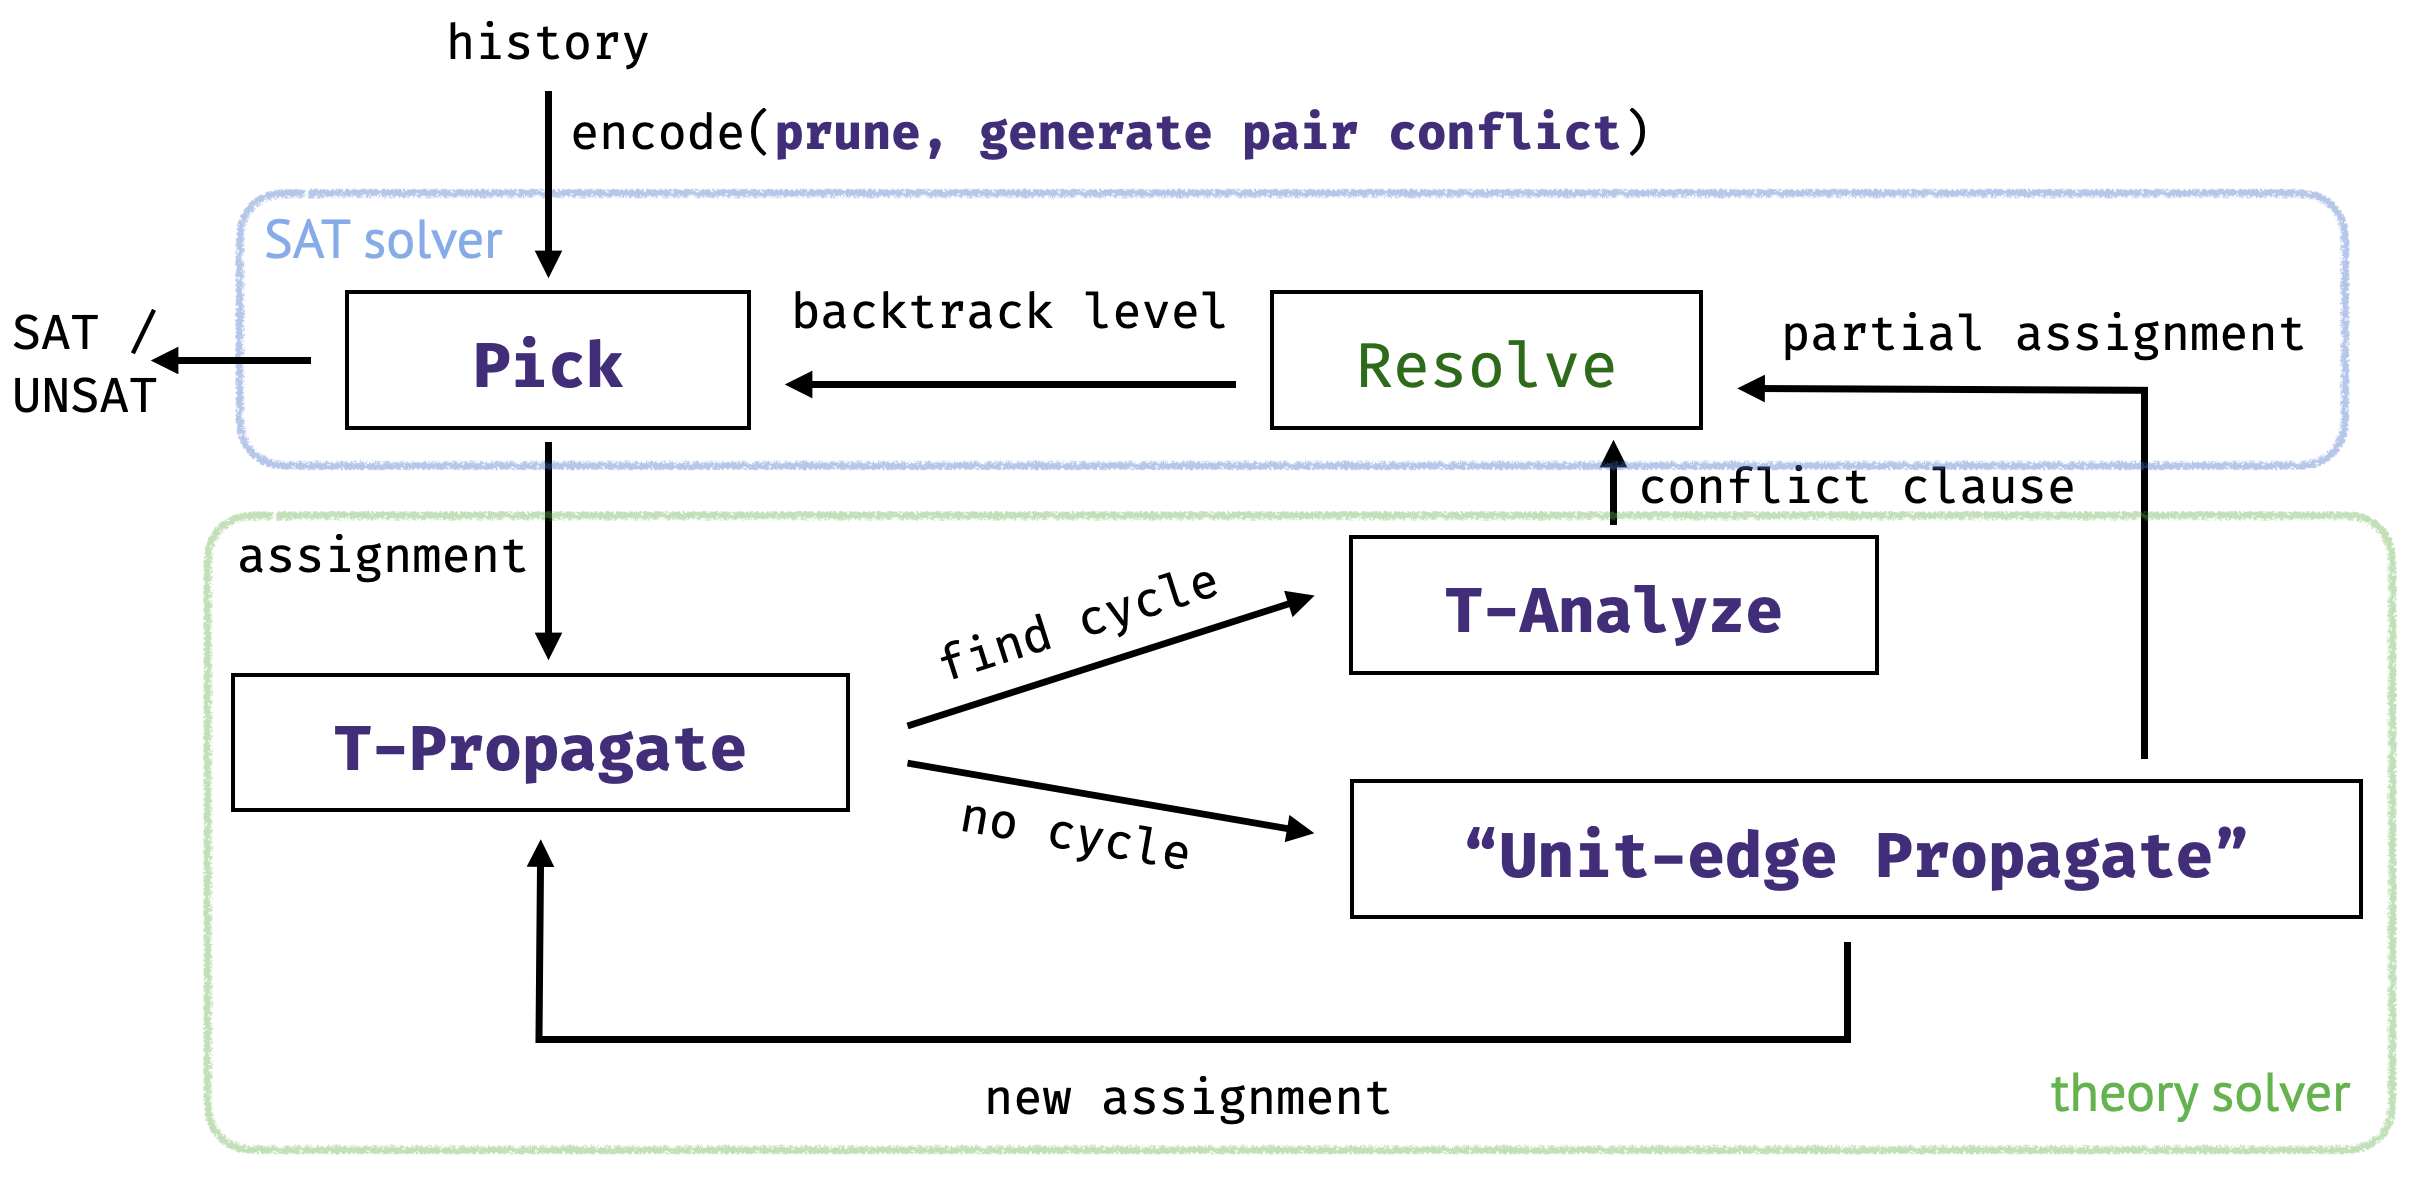
\includegraphics[width=0.45\textwidth]{figs/acyclic-minisat-framework}}
	% 	\subfigure[name2]{
	% 	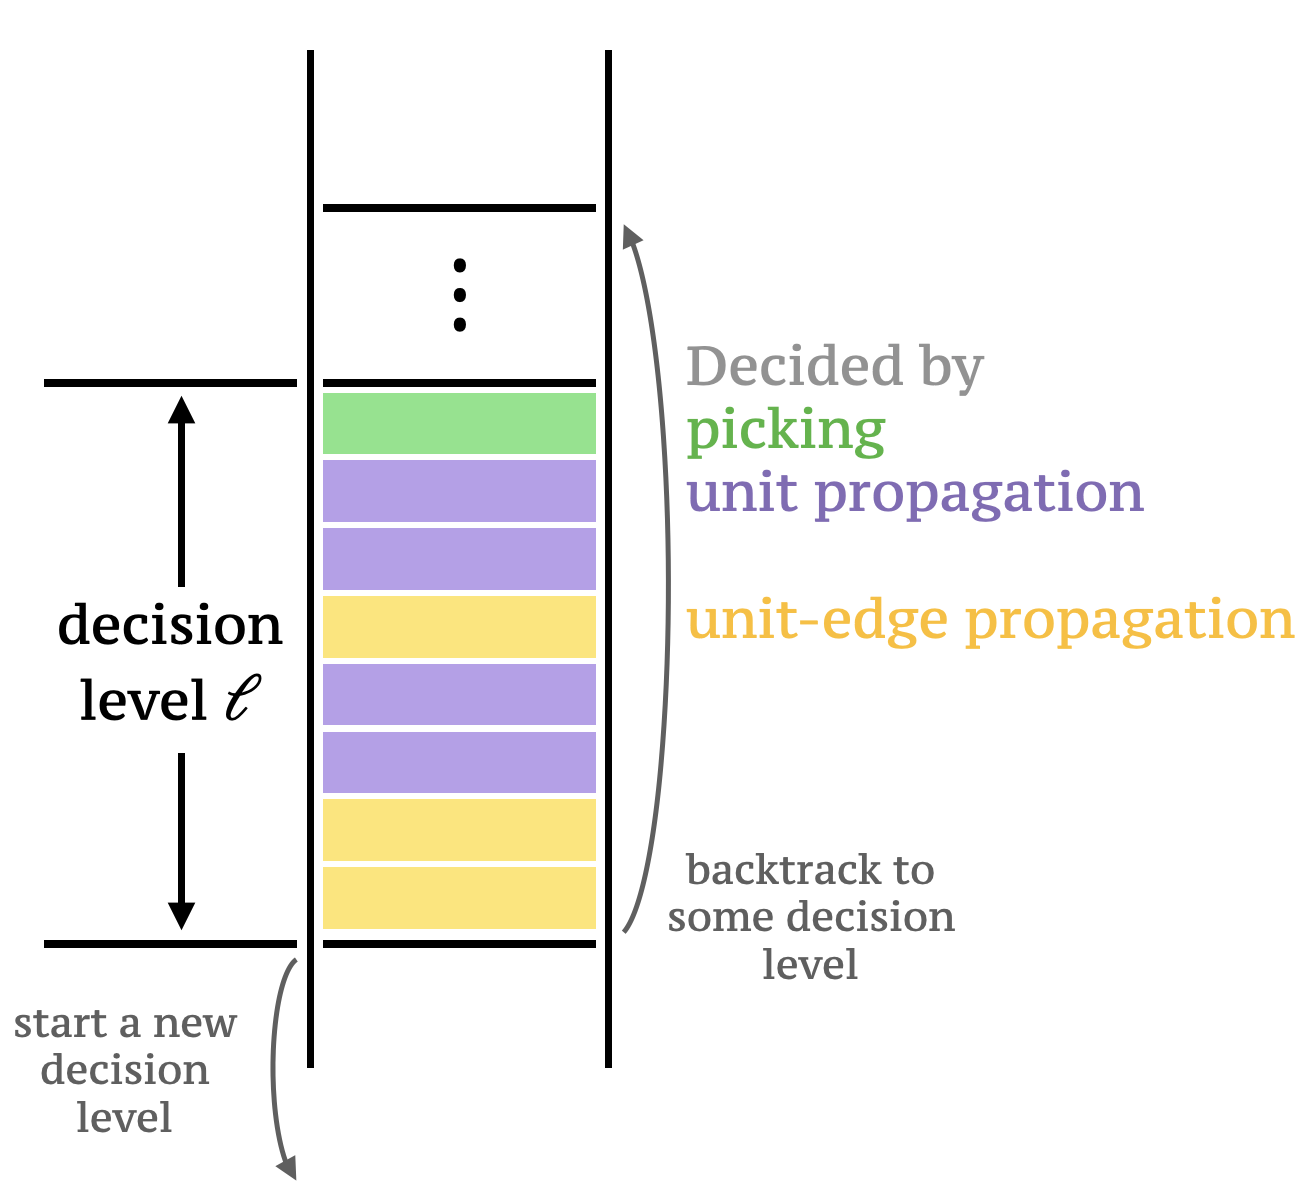
\includegraphics[width=0.45\textwidth]{figs/acyclic-minisat-decision-trail}}
	% \end{figure}

	\begin{figure}[H]
		\centering
		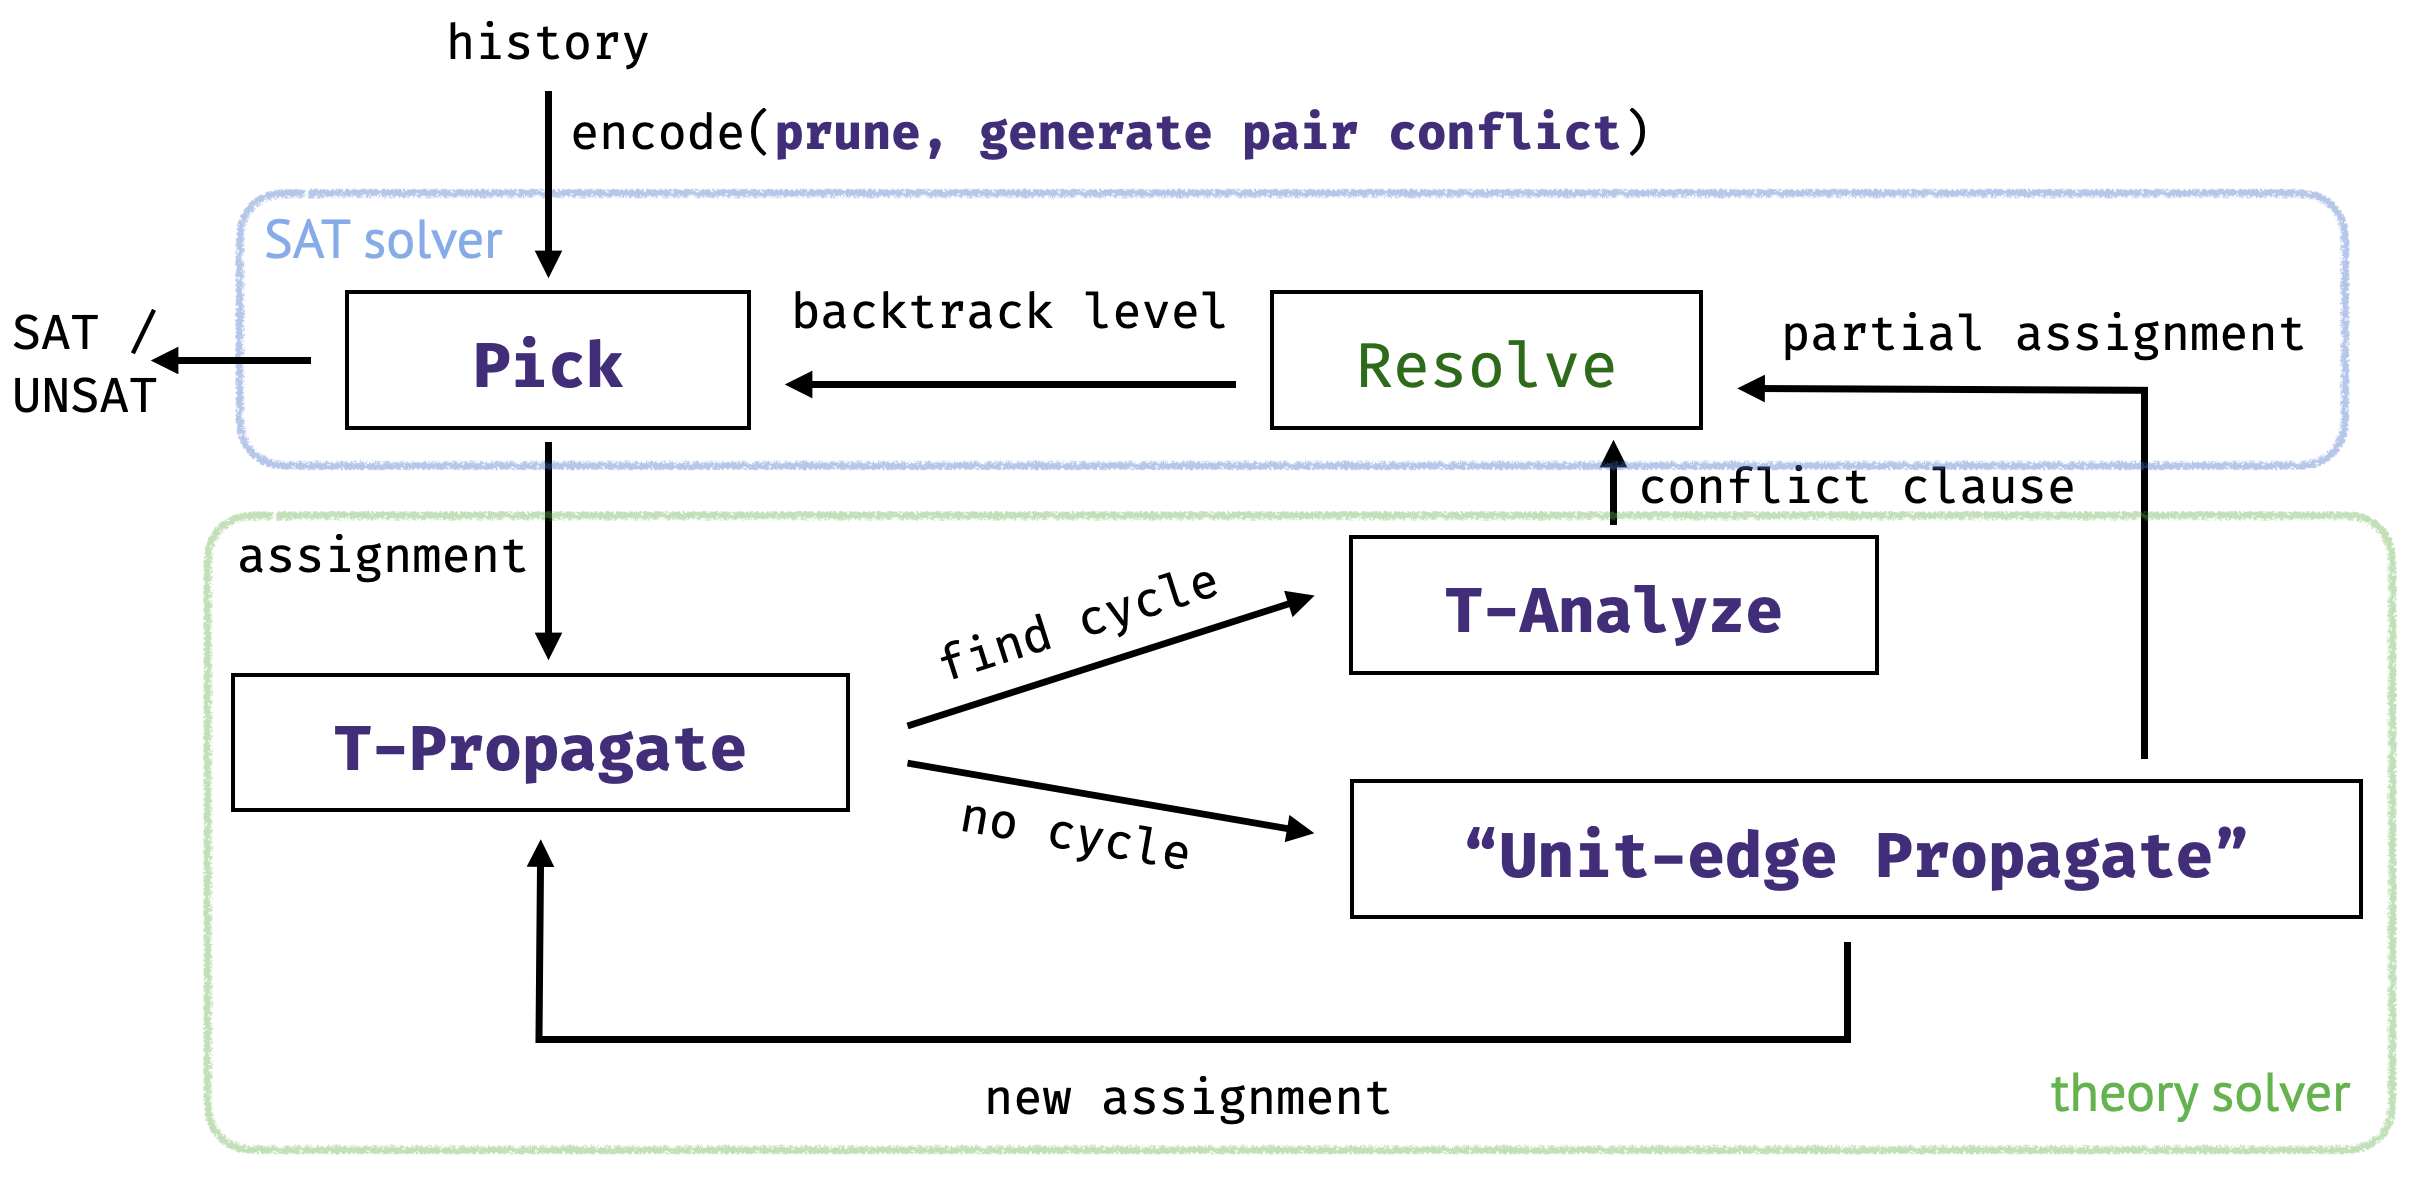
\includegraphics[width=0.6\textwidth]{figs/acyclic-minisat-framework.png}~
		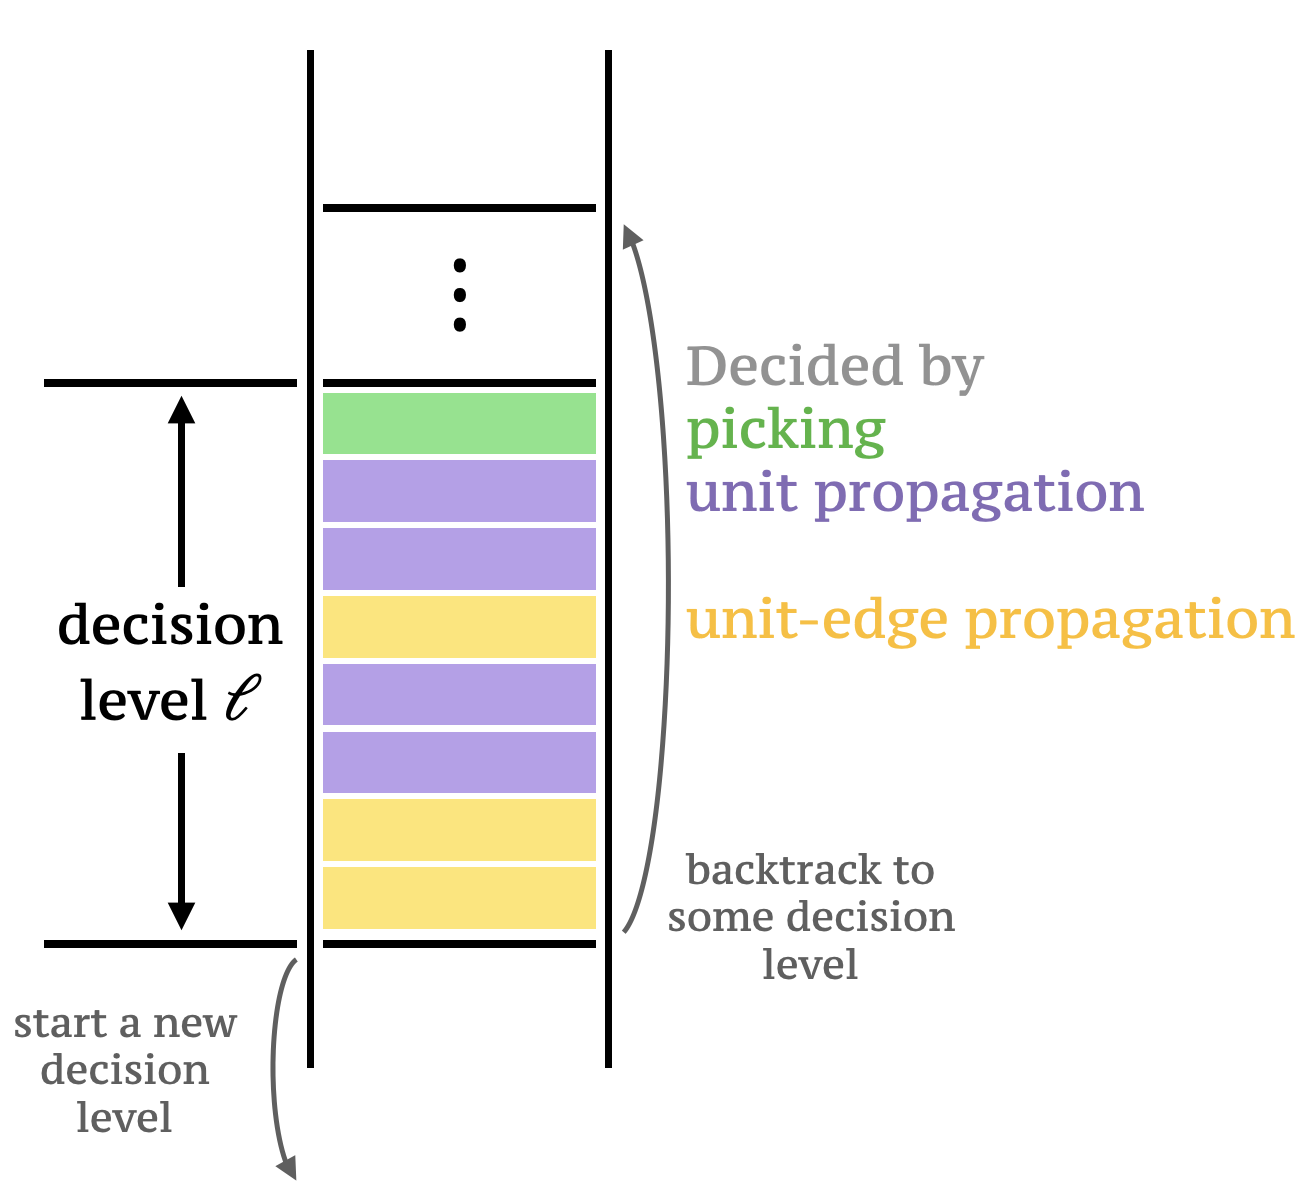
\includegraphics[width=0.36\textwidth]{figs/acyclic-minisat-decision-trail.png}
		\vspace*{0.30cm}
		\footnotesize{framework(left) and decision trail(right)}
	\end{figure}

	% \textcolor[RGB]{71,46,125}{\textbf{#1}}}
	\footnotesize{\textcolor[RGB]{71,46,125}{\textbf{Possible optimizations:}}}
	\scriptsize{
		\begin{itemize}
			\item \textcolor[RGB]{71,46,125}{\textbf{Pick}}: select a variable to make an assignment
			\item \textcolor[RGB]{71,46,125}{\textbf{T}}heory\textcolor[RGB]{71,46,125}{\textbf{-Propagate}}: efficiently detect possible cycle upon inserting arcs
			\item \textcolor[RGB]{71,46,125}{\textbf{T}}heory\textcolor[RGB]{71,46,125}{\textbf{-Analyze}}: find proper cycle(s)
			\item \textcolor[RGB]{71,46,125}{\textbf{Unit-edge Propagate}}: derive literatures from current reachability
		\end{itemize}
	}
\end{frame}
%%%%%%%%%%%%%%%%%%%%%%%%%%%%%%

%%%%%%%%%%%%%%%%%%%%%%%%%%%%%%
\begin{frame}{Optimization 1}{ICD algorithm and unit-edge propagation}
	\blue{I}ncermental \blue{C}ycle \blue{D}etection Algorithm
	\begin{itemize}
		\item is a two-way search algorithm for sparse graphs.
		\item takes at most $O(\min\{m^{1/2}, n^{2/3}\}m)$ time to insert $m$ arcs into an $n$-vertex graph.
	\end{itemize}

	\begin{figure}[H]
		\centering
		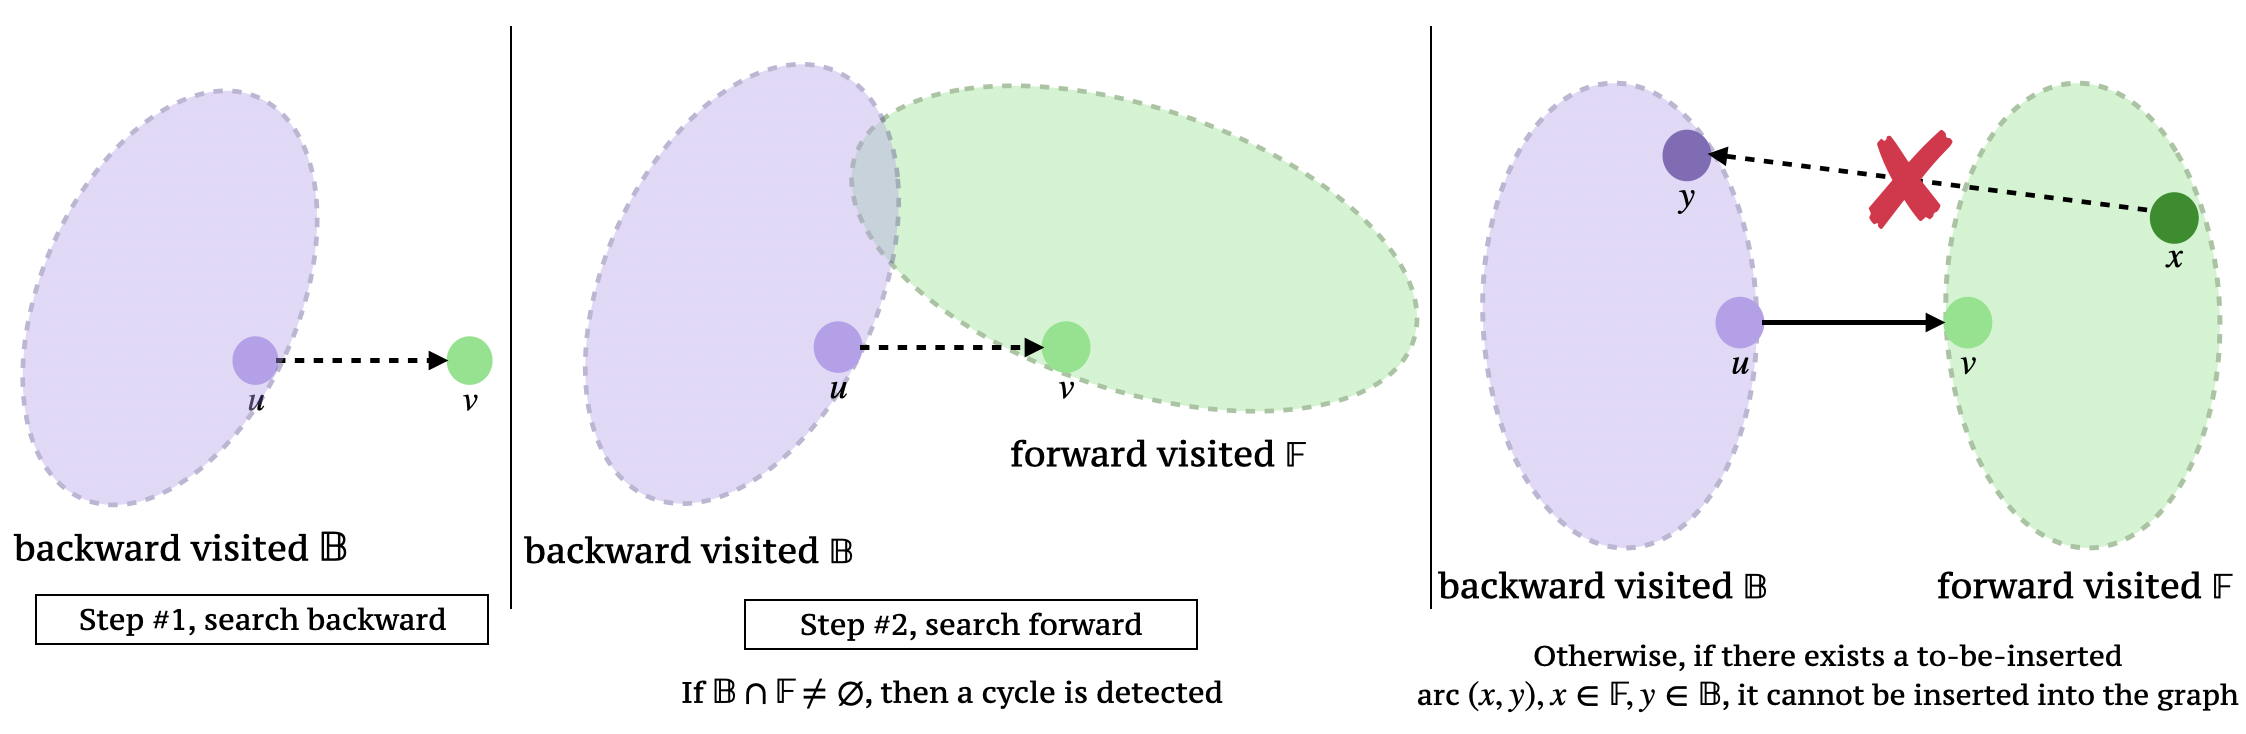
\includegraphics[width=\textwidth]{figs/ICD-algorithm-and-unit-edge-propagation.png}
	\end{figure}

	\begin{itemize}
		\item iterate on each inactive arc $(x, y)$ , then some values can be decided instantly(\blue{Unit-edge Propagation}). 
	\end{itemize}
\end{frame}
%%%%%%%%%%%%%%%%%%%%%%%%%%%%%%

%%%%%%%%%%%%%%%%%%%%%%%%%%%%%%
\begin{frame}{Optimization 2}{pruning, pair conflict generation, ...}
	\scriptsize{
		\begin{itemize}
			\item for a simple constraint $C = \{C_1, C_2\} = \{\{(x, y)\}, \{(y, x)\}\}$, if it is reachable from $y$ to $x$, then $C_2 = \{(y, x)\}$ must be inserted into the graph(\blue{Pruning}).
			\item Observation: after pruning, the average width\footnote{\tiny{number of different variables on a cycle}} of detected cycles is $\in [2, 3)$, which means most conflict clauses only consist of 2 variables.
			\item Such clauses can be generated beforewise(\blue{Pair Conflict Generation}).
		\end{itemize}
	}

	\begin{figure}[H]
		\centering
		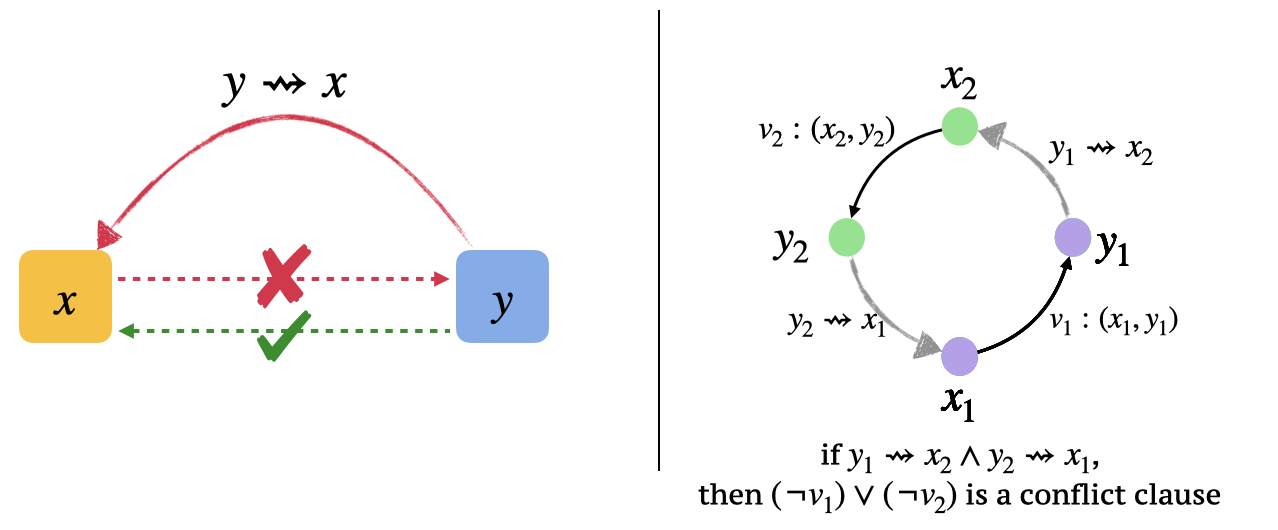
\includegraphics[width=0.8\textwidth]{figs/pruning-and-pair-conflict-generation.png}
	\end{figure}

	\begin{itemize}
		\item maybe a hint: Pruning handles 1-width cycles, pair conflict generation handles 2-width cycles, now the average width has come to $[3, 4)$ ...
	\end{itemize}
\end{frame}
%%%%%%%%%%%%%%%%%%%%%%%%%%%%%%

%%%%%%%%%%%%%%%%%%%%%%%%%%%%%%
\begin{frame}{Experimental Evaluation}
	% \begin{center}
	% 	\scriptsize{
	% 		\begin{tabular}{|c|c|c|c|c|}
	% 			\hline
	% 			baseline & \makecell{cycle\\ detection} & \makecell{conflict\\ generation} & \makecell{unit-edge\\ propagation} & \makecell{pair conflict\\generation} \\
	% 			\hline
	% 			z3 user propagator* & local toposort & smallest & $\checkmark$(partial) & \\
	% 			\hline
	% 			monosat & PK toposort & first & & \\
	% 			\hline
	% 			acyclic minisat* & ICD & first & $\checkmark$ & $\checkmark$ \\
	% 			\hline
	% 			cobra(w/o GPU) & \multicolumn{3}{c|}{same as monosat} & \\
	% 			\hline 
	% 		\end{tabular} 
	% 	}
	% 	\\
	% 	\tiny{*: we implemented}
	% \end{center}

	\begin{figure}[H]
		\centering
		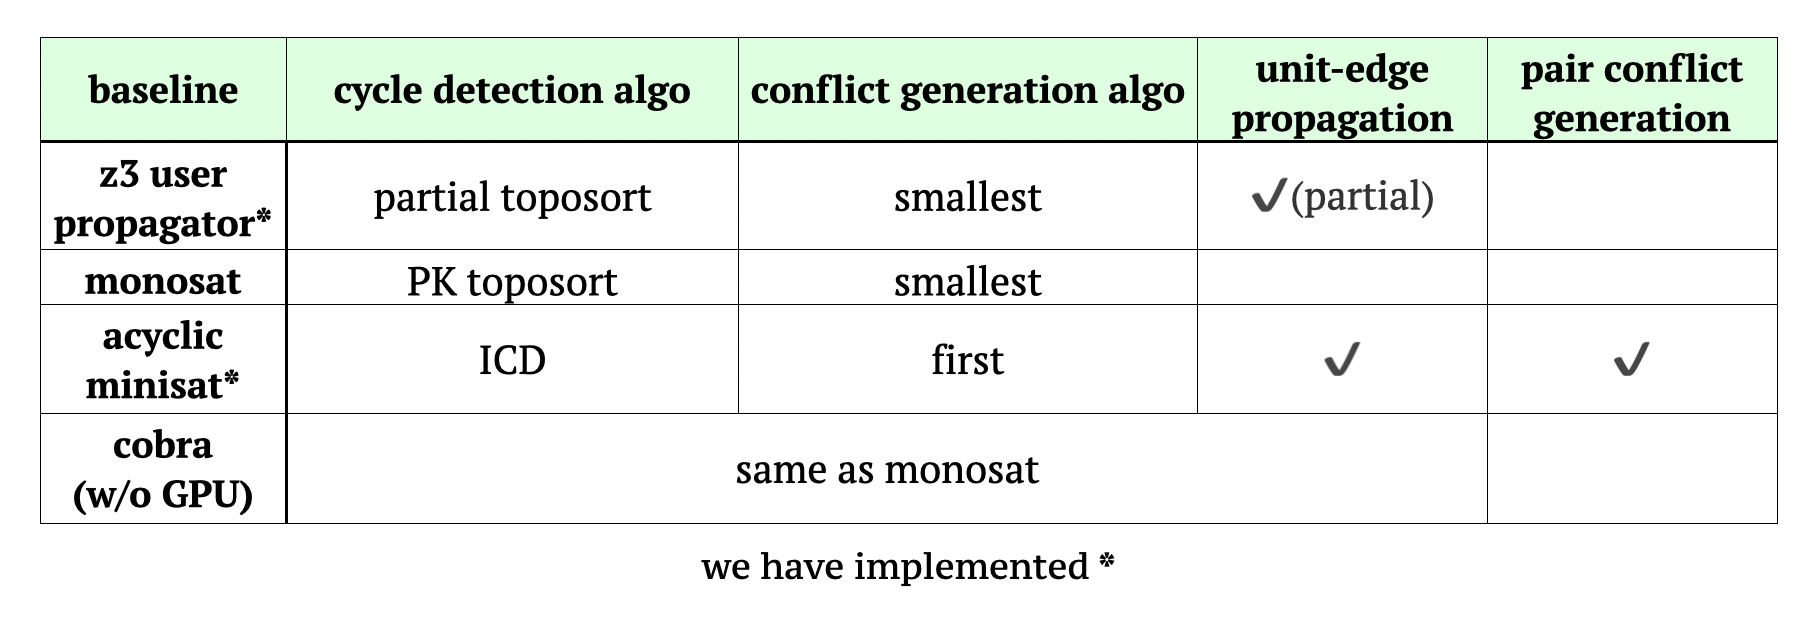
\includegraphics[width=\textwidth]{figs/ser-checker-baselines.png}		
	\end{figure}
	
\end{frame}

\begin{frame}{Experimental Evaluation}
	\begin{figure}[H]
		\centering
		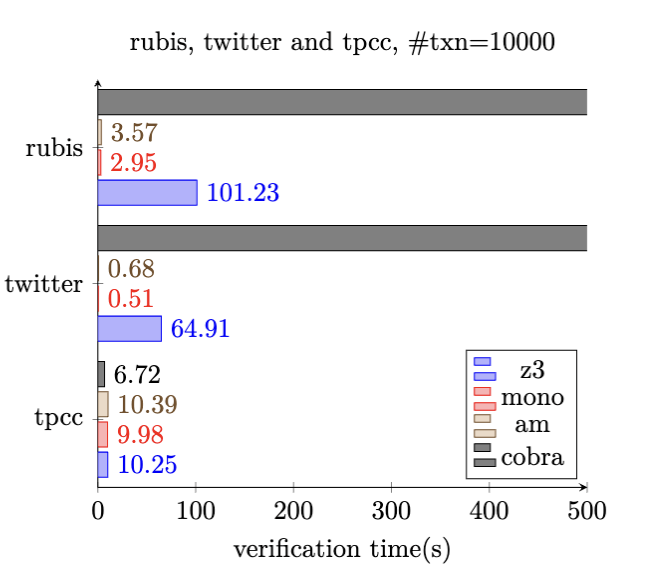
\includegraphics[width=0.48\textwidth]{figs/ser-checker-rubis-twitter-and-tpcc-ntxn10000.png}
		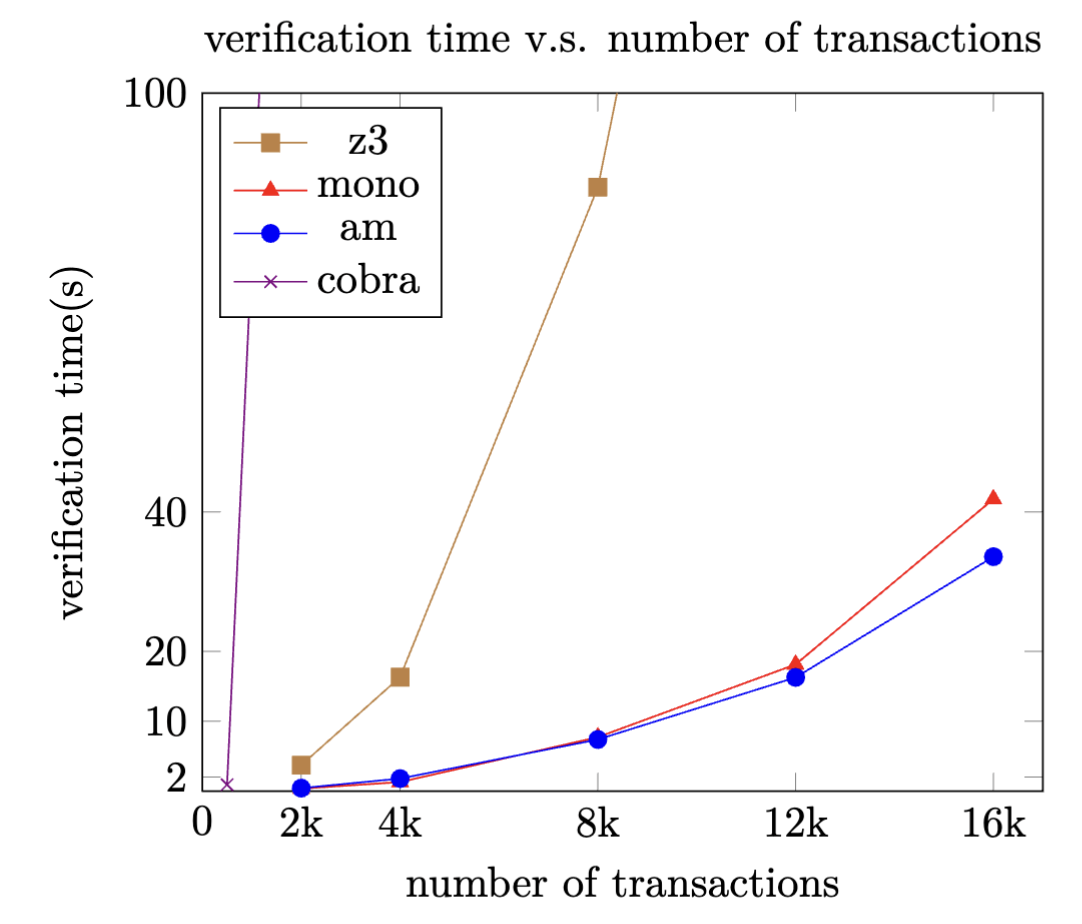
\includegraphics[width=0.48\textwidth]{figs/ser-checker-chengRW-verification-time-vs-ntxns.png}
	\end{figure}
\end{frame}
%%%%%%%%%%%%%%%%%%%%%%%%%%%%%%

%%%%%%%%%%%%%%%%%%%%%%%%%%%%%%
\begin{frame}{What Needs To Do Next}
	what needs to do next
\end{frame}
%%%%%%%%%%%%%%%%%%%%%%%%%%%%%%

%%%%%%%%%%%%%%%%%%%%%%%%%%%%%%
\begin{frame}
	extended to client program verification and robustness verification
\end{frame}
%%%%%%%%%%%%%%%%%%%%%%%%%%%%%%